\chapter{Chapter name here (title of the paper)}
\label{art1:ch:article_1}

\dictum[James C. Maxwell]{%
  Some wise words}%
\vskip 1em

\textit{\large{Authors, separated by comma}}
\bigskip
\bigskip

A version of this paper has been submitted to \textit{Journal name} (ISSN 469-7696).
\bigskip

I have presented it at:

\begin{itemize}
    \setlength{\itemsep}{0pt}
    \setlength{\parskip}{0pt}
    \setlength{\parsep}{0pt}
    \item[--] PhD Workshop on Quantitative Finance and Econometrics, July 2019, Manchester, UK;
    \item[--] Quantitative Finance and Financial Econometrics 2018, June 2018, Marseille, France.
\end{itemize}
\bigskip

\section*{Abstract}
\label{art1:sec:Abstract}
Your abstract for this paper

%////////////////////////////////////////////////////////////////%

\section{Introduction}
\label{art1:sec:Introduction}
Text here \citep{dacorogna2001extremal}.

\section{Intrinsic Time}
\label{art1:sec:IntrinsicTime}

%
\begin{figure}
\begin{center}
\begin{minipage}{160mm}
\resizebox*{160mm}{!}{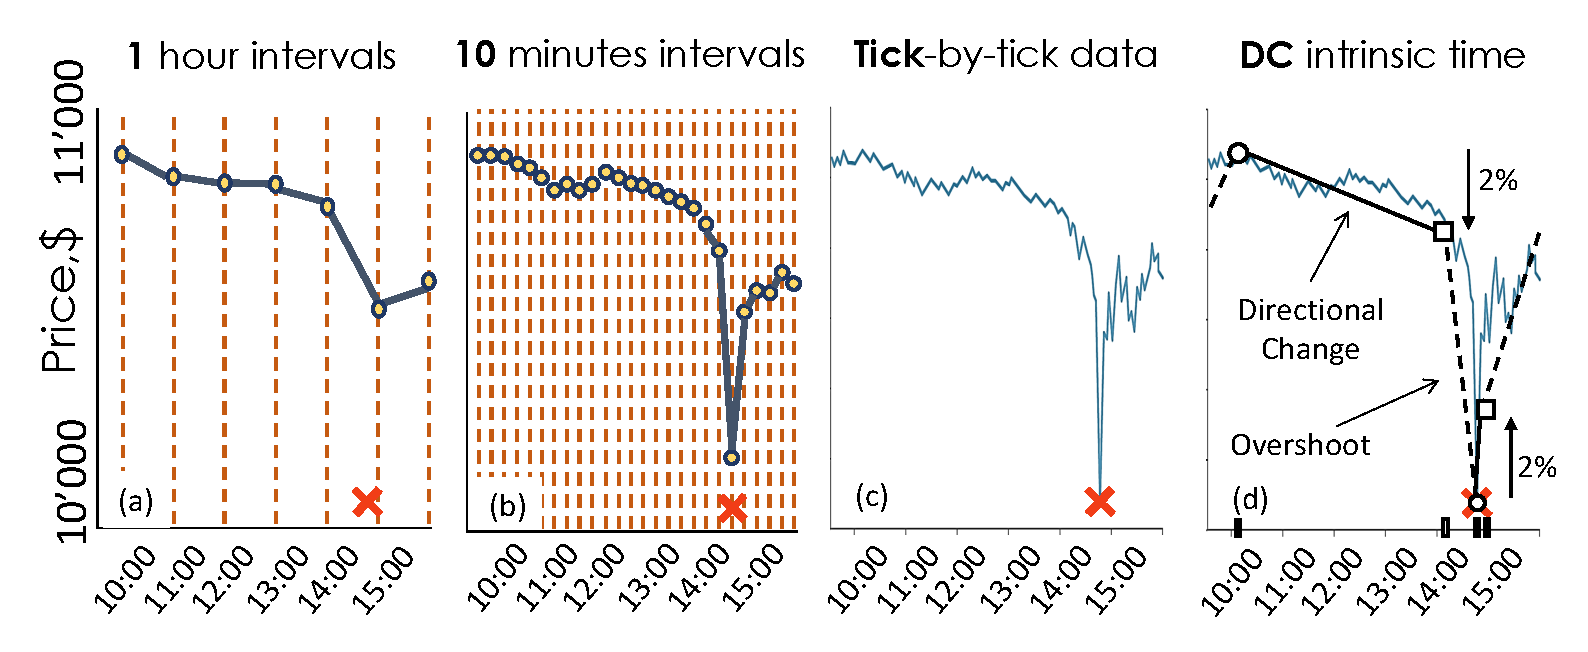
\includegraphics{uzh-thesis-master/chapters/article_1/Pictures/Flash_crash.pdf}}
\caption{Example of a picture.
\label{art1:fig:dissect_price}}
\end{minipage}
\end{center}
\end{figure}

%
\begin{equation}
    N(\delta) = \left( \frac{\delta}{C} \right)^{E},
\end{equation}
%

\begin{figure}[h!]
\centering
    \begin{subfigure}{0.45\textwidth}
        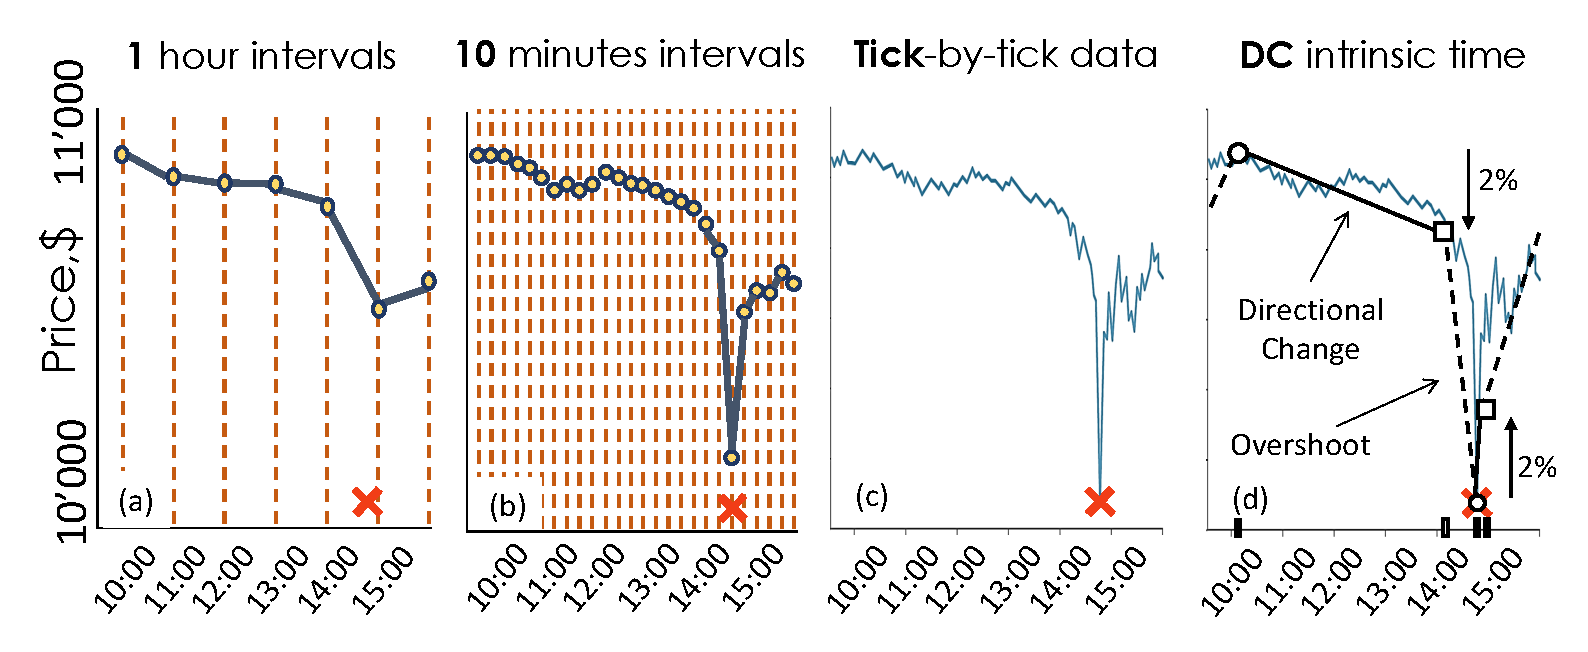
\includegraphics[width=0.9\linewidth]{uzh-thesis-master/chapters/article_1/Pictures/Flash_crash.pdf}
        \caption{}
        \label{art1:fig:acf_returns}
    \end{subfigure}
    \begin{subfigure}{0.45\textwidth}
        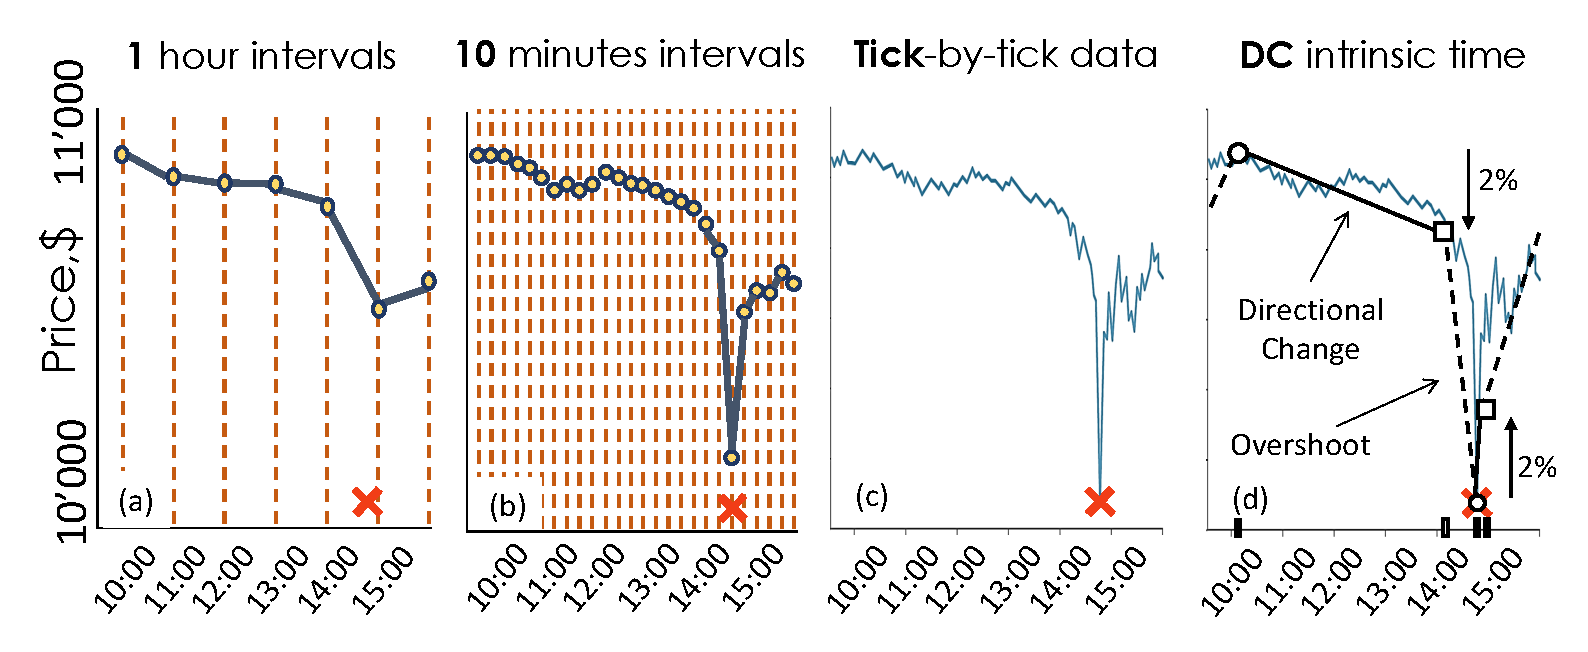
\includegraphics[width=0.9\linewidth]{uzh-thesis-master/chapters/article_1/Pictures/Flash_crash.pdf}
        \caption{}
        \label{art1:fig:acf_absolute_returns}
    \end{subfigure}
    \caption[]{Several pictures}
    \label{art1:fig:ACF_properties}
\end{figure}


%////////////////////////////////////////////////////////////////%
 
\begin{subappendices}
\newpage
\section{Overshoot as the Function of Trend}
\label{art1:appendix:OvershootTrend}
Some text

\section{Dissection Algorithm}
\label{art1:appendix:DissectAlgo}
Some text
 
\end{subappendices}
 
 
\clearpage
